\section{Radiation pressure modeling for LRO}

TODO write intro

\subsection{Lunar albedo radiation}
\label{subsec:lunar-albedo}

\begin{figure*}[t]
    \centering

    \begin{subfigure}[c]{0.49\textwidth}
        \includegraphics[width=\textwidth]{figures/plots/lunar_map_photo.pdf}
    \end{subfigure}
    \hfill
    \begin{subfigure}[c]{0.49\textwidth}
        \includegraphics[width=\textwidth]{figures/plots/lunar_map_dlam1.pdf}
    \end{subfigure}
    
    \bigskip
    
    \begin{subfigure}[c]{0.49\textwidth}
        \includegraphics[width=\textwidth]{figures/plots/lunar_hist_photo.pdf}
        \subcaption{Mosaic (mean = 0.12, minimum = 0.05, 99th percentile = 0.29)~\cite{UASC2009}}
        \label{fig:lunar-albedo-map-photo}
    \end{subfigure}
   \hfill
    \begin{subfigure}[c]{0.49\textwidth}
        \includegraphics[width=\textwidth]{figures/plots/lunar_hist_dlam1.pdf}
        \subcaption{\acrshort{DLAM1} (mean = 0.15, minimum = 0.04, 99th percentile = 0.22)}
        \label{fig:lunar-albedo-map-dlam1}
    \end{subfigure}

   \caption{Lunar albedo distribution from Clementine. Both the mosaic and \acrshort{DLAM1} are based on 750 nm reflectivity, but \acrshort{DLAM1} has been corrected to the average solar wavelength. Large bright features like the Tycho and Giordano Bruno craters (\textcolor{mpl-pink}{\ding{108}}) can be registered. Note that the maximum of the albedo scale here is 0.5 instead of 1.0 to increase contrast; in reality, the Moon appears half as bright.}
   \label{fig:lunar-albedo-map}
\end{figure*}

The Moon is a major source of radiation in \gls{LRO}'s orbit, with lunar irradiance magnitudes approaching half of the Sun's. Therefore, albedo and thermal radiation due to the Moon will be modeled. While the lunar albedo is only \qty{40}{\percent} of Earth's albedo~\cite{Goode2001}, albedo radiation due to the Moon is still substantial, particularly over the subsolar point~\cite{Floberghagen1999}. Lunar albedo varies significantly with geology: the highlands (mean $a = 0.16$, maximum $a=0.25$) are much more reflective than the maria (mean $a = 0.07$, minimum $a = 0.05$) due to their respective regolith composition~\cite{Vasavada2012,Hayne2017,Sato2014}. The mosaic of calibrated albedo imagery from Clementine in \cref{fig:lunar-albedo-map-photo} clearly shows the differences between highlands and marias. The mean of 0.12 agrees with other literature~\cite{Vasavada2012}, and most of the lunar surface has an albedo below 0.20. Higher values are only found at the poles, where the imagery represents topographic shading rather than actual albedo~\cite{McEwen1997}. Note that the mosaic is for albedo of light at \qty{750}{\nm} wavelength, which is slightly longer than the average solar wavelength. Even though solar radiation has most energy within the \qtyrange{300}{2400}{\nm} band, the spectrum peaks at around \qty{470}{\nm}~\cite{Iqbal1983}. Lunar reflectivity increases with increasing wavelength~\cite{Shkuratov2011}.

\citeauthor{Floberghagen1999}'s \numproduct{15x15} spherical harmonics expansion called \gls{DLAM1}~\cite{Floberghagen1999} is often used to represent this spatial albedo variability in lunar \gls{RP} models. \gls{DLAM1} was fitted from Clementine imagery and was designed to work with Knocke's albedo model for dynamic paneling (\cref{eq:radiosity-albedo}). Due to the nature of spherical harmonics, the model cannot resolve features smaller than \ang{12} (\qty{360}{\km} at the equator). The expansion is shown in \cref{fig:lunar-albedo-map-dlam1}, along with direct imagery from Clementine. \gls{DLAM1} was also derived from 750 nm imagery, but we scale the original values by $1/1.3$ to account for the reduced reflectivity at the average solar solar wavelength. This factor was proposed by \citeauthor{Vasavada2012}~\cite{Vasavada2012}. Even with the correction, the mean albedo of the expansion of 0.15 is still \qty{25}{\percent} above the commonly accepted mean of 0.12. This is possibly due to a different calibration of the imagery that \gls{DLAM1} is based on compared to the mosaic from \cref{fig:lunar-albedo-map-photo}. In fact, Clementine is known to overestimate albedo due to bad calibration~\cite{Shkuratov2011}. Apart from the difference in magnitude, the patterns agree reasonably well: maria and highlands are distinct and large bright features like the ray system around the Tycho and Giordano Bruno craters can be recognized (marked in \cref{fig:lunar-albedo-map-dlam1}).

Despite the shortcomings of \gls{DLAM1}, spherical harmonics are convenient: they are smooth and do not require interpolation like a gridded map. They can easily be truncated to trade detail for computational efficiency. Therefore, we will use \gls{DLAM1} in this paper but consider that the magnitude may be overestimated by \qty{25}{\percent} during the analysis of results. We will also compare results for the location-dependent \gls{DLAM1} with those for a constant value, which should be more computationally efficient. As single representative albedo, we choose the mean of 0.15 instead of 0.12 to facilitate comparison. Note that the spatial variability described above suggests that a single albedo value cannot accurately represent lunar reflectivity.

Albedo radiation assumes ideal, diffuse Lambertian reflectance, which decreases with the cosine of the viewing angle. This assumption is especially appropriate for Earth, for which purely specular radiosity only amounts to \qty{10}{\percent} of the purely diffuse radiosity~\cite{Knocke1988}. However, this is not the case for the Moon: the opposition effect increases the reflectance at low phase angles (when the source is behind the observer, see \cref{fig:eclipse-geometry}) much more than would be expected from a cosine law. In fact, the brightness increases more than \qty{40}{\percent} between phase angles of \ang{4} and \ang{0}~\cite{Buratti1996}. This is primarily caused by shadow hiding. To account for non-diffuse reflectance of the lunar surface, the Hapke \gls{BRDF} was developed~\cite{Hapke2012}. This \gls{BRDF} is an empirical relation based on nine parameters that control, among other phenomena, the strength and directionality of the opposition effect. Near-global maps for these parameters have been fitted from \gls{LRO} observations and could be used for a radiosity model~\cite{Sato2014}. For \gls{RP} acceleration modeling, the opposition effect is only of concern when the target is above the subsolar point; the Sun has to be in the orbital plane for this. For \gls{LRO}, this only occurs for a few days twice a year, and even then only for a small fraction of the orbit. Therefore, we will neglect opposition effect in this study.




\subsection{Lunar thermal radiation}

Lunar surface temperatures and the associated thermal radiation undergoes a significant diurnal cycle. Daytime and nighttime temperatures can differ by up to \qty{290}{\K}. The surface heats rapidly after sunrise, cools at about the same rate after local noon, then slower during the night~\cite{Vasavada2012}. There are small seasonal changes, with the noon temperature differing by \qty{6}{\K} between lunar aphelion and perihelion~\cite{Heiken1991}. The large diurnal variability makes Knocke's delayed thermal model (\cref{eq:radiosity-thermal-delayed}), which gives a constant radiosity throughout the day, unsuitable for the Moon.

Diurnal variability is represented well by the angle-based thermal model (\cref{eq:radiosity-thermal-anglebased}). We parametrize the model with the equatorial temperatures just before sunrise ($T_\textnormal{min} = \qty{95}{\K}$) and at local noon ($T_\textnormal{max} = \qty{385}{\K}$). The model transitions to the nighttime temperature when the incidence angle $\theta_i \geq \ang{89.8}$. The temperatures span a slightly larger range than \citeauthor{Lemoine2013} ($T_\textnormal{min} = \qty{100}{\K}, T_\textnormal{max} = \qty{375}{\K}$), who initially proposed the angle-based model. However, they agree with those used by \citeauthor{Park2011}~\cite{Park2011}. Note that \citeauthor{Park2011}'s model is identical up to a factor $1/4$ in the radiosity, which is incorrect.

While the albedo varies with location (see \cref{subsec:lunar-albedo}), the emissivity and other thermophysical properties are remarkably uniform~\cite{Hayne2017}. This means that a constant emissivity is a fair assumption. We use a value of $e = 0.95$, which is the broadband daytime emissivity, although it decreases to 0.90 during the night~\cite{Bandfield2015}. However, we assume the constant daytime emissivity at all times.

\begin{figure}[t]
    \centering
    \includegraphics[width=\linewidth]{figures/plots/thermal_map.pdf}
    \caption{Map of lunar thermal emissions from the angle-based model (\cref{eq:radiosity-thermal-anglebased}). The emissivity is 0.95 and surface temperatures range between \qty{95}{\K} and \qty{385}{\K}, depending on the subsolar angle.}
    \label{fig:thermal-map}
\end{figure}

The thermal surface radiosity $J_\textnormal{thermal}$ from the angle-based model with the aforementioned parameters is shown in \cref{fig:thermal-map}. The radiosity decreases with the cosine of the incidence angle and approaches negligible emissions of \qty{6}{\irr} at nighttime. The maximum radiosity, which occurs below the subsolar point (i.e., at local noon), is \qty{1246}{\irr}. This peak value agrees with those used to design \gls{LRO}'s thermal control subsystem~\cite{Tooley2010}. The only effect that is not captured is the slow cooling by about \qty{25}{\K} between sunset and sunrise~\cite{Vasavada2012}, which introduces a slight asymmetry; we use constant pre-sunrise temperatures throughout the night. We also do not model seasonal variations of surface temperature.





\subsection{Paneling of the Moon}

Knocke's dynamic paneling method described in \cref{subsec:radiation-sources} will be used for the Moon. \gls{LRO}'s low altitude compared to the lunar radios prohibits any static paneling, which would have a large number of never-visible panels.

\begin{figure}[t]
    \centering
    \includegraphics[width=\linewidth]{figures/plots/paneling_convergence.pdf}
    \caption{Convergence of lunar irradiance received by \gls{LRO} for increasing number of rings. Each ring contains six more panels than the previous. Six rings (\textcolor{mpl-red}{\textbf{---}}) are sufficient for an error of less than \qty{10}{\percent} with respect to the converged solution.}
    \label{fig:paneling-convergence}
\end{figure}

Selecting the number of rings is a trade-off between fidelity and computational efficiency. To determine the lowest number of rings that can still represent lunar radiation with sufficient accuracy, we investigated the convergence behavior. \Cref{fig:paneling-convergence} shows the albedo and thermal irradiance received by \gls{LRO} for an increasing number of rings. As suggested by \citeauthor{Knocke1988}, each ring contains six more panels than the previous one. For 13 rings and more, the peak irradiance is within \qty{1}{\percent} of \qty{1687}{\irr}. For six rings, the irradiance peaks at \qty{1540}{\irr}, which is within \qty{10}{\percent} of the converged solution. The results are similar for constant and \gls{DLAM1} albedo.

We choose six rings as sufficiently accurate, which contain 127 panels in total. The panel geometry in this case was already shown in \cref{fig:general-knocke-paneling-low}. This is one ring (or 36 panels) more than used by others. \citeauthor{Floberghagen1999} suggests five rings for Lunar Prospector, which has twice the orbital altitude of \gls{LRO} and thus needs fewer rings (\citeauthor{Knocke1988} only used two rings for a much higher altitude relative to the planetary radios). Five rings are also used for \gls{LRO}'s operational orbit determination~\cite{Nicholson2010}. We choose one ring more to keep the error due to paneling below \qty{10}{\percent}. A higher number may be required in case of a higher-resolution albedo distribution




\subsection{LRO target}

\begin{figure}[t]
    \centering
    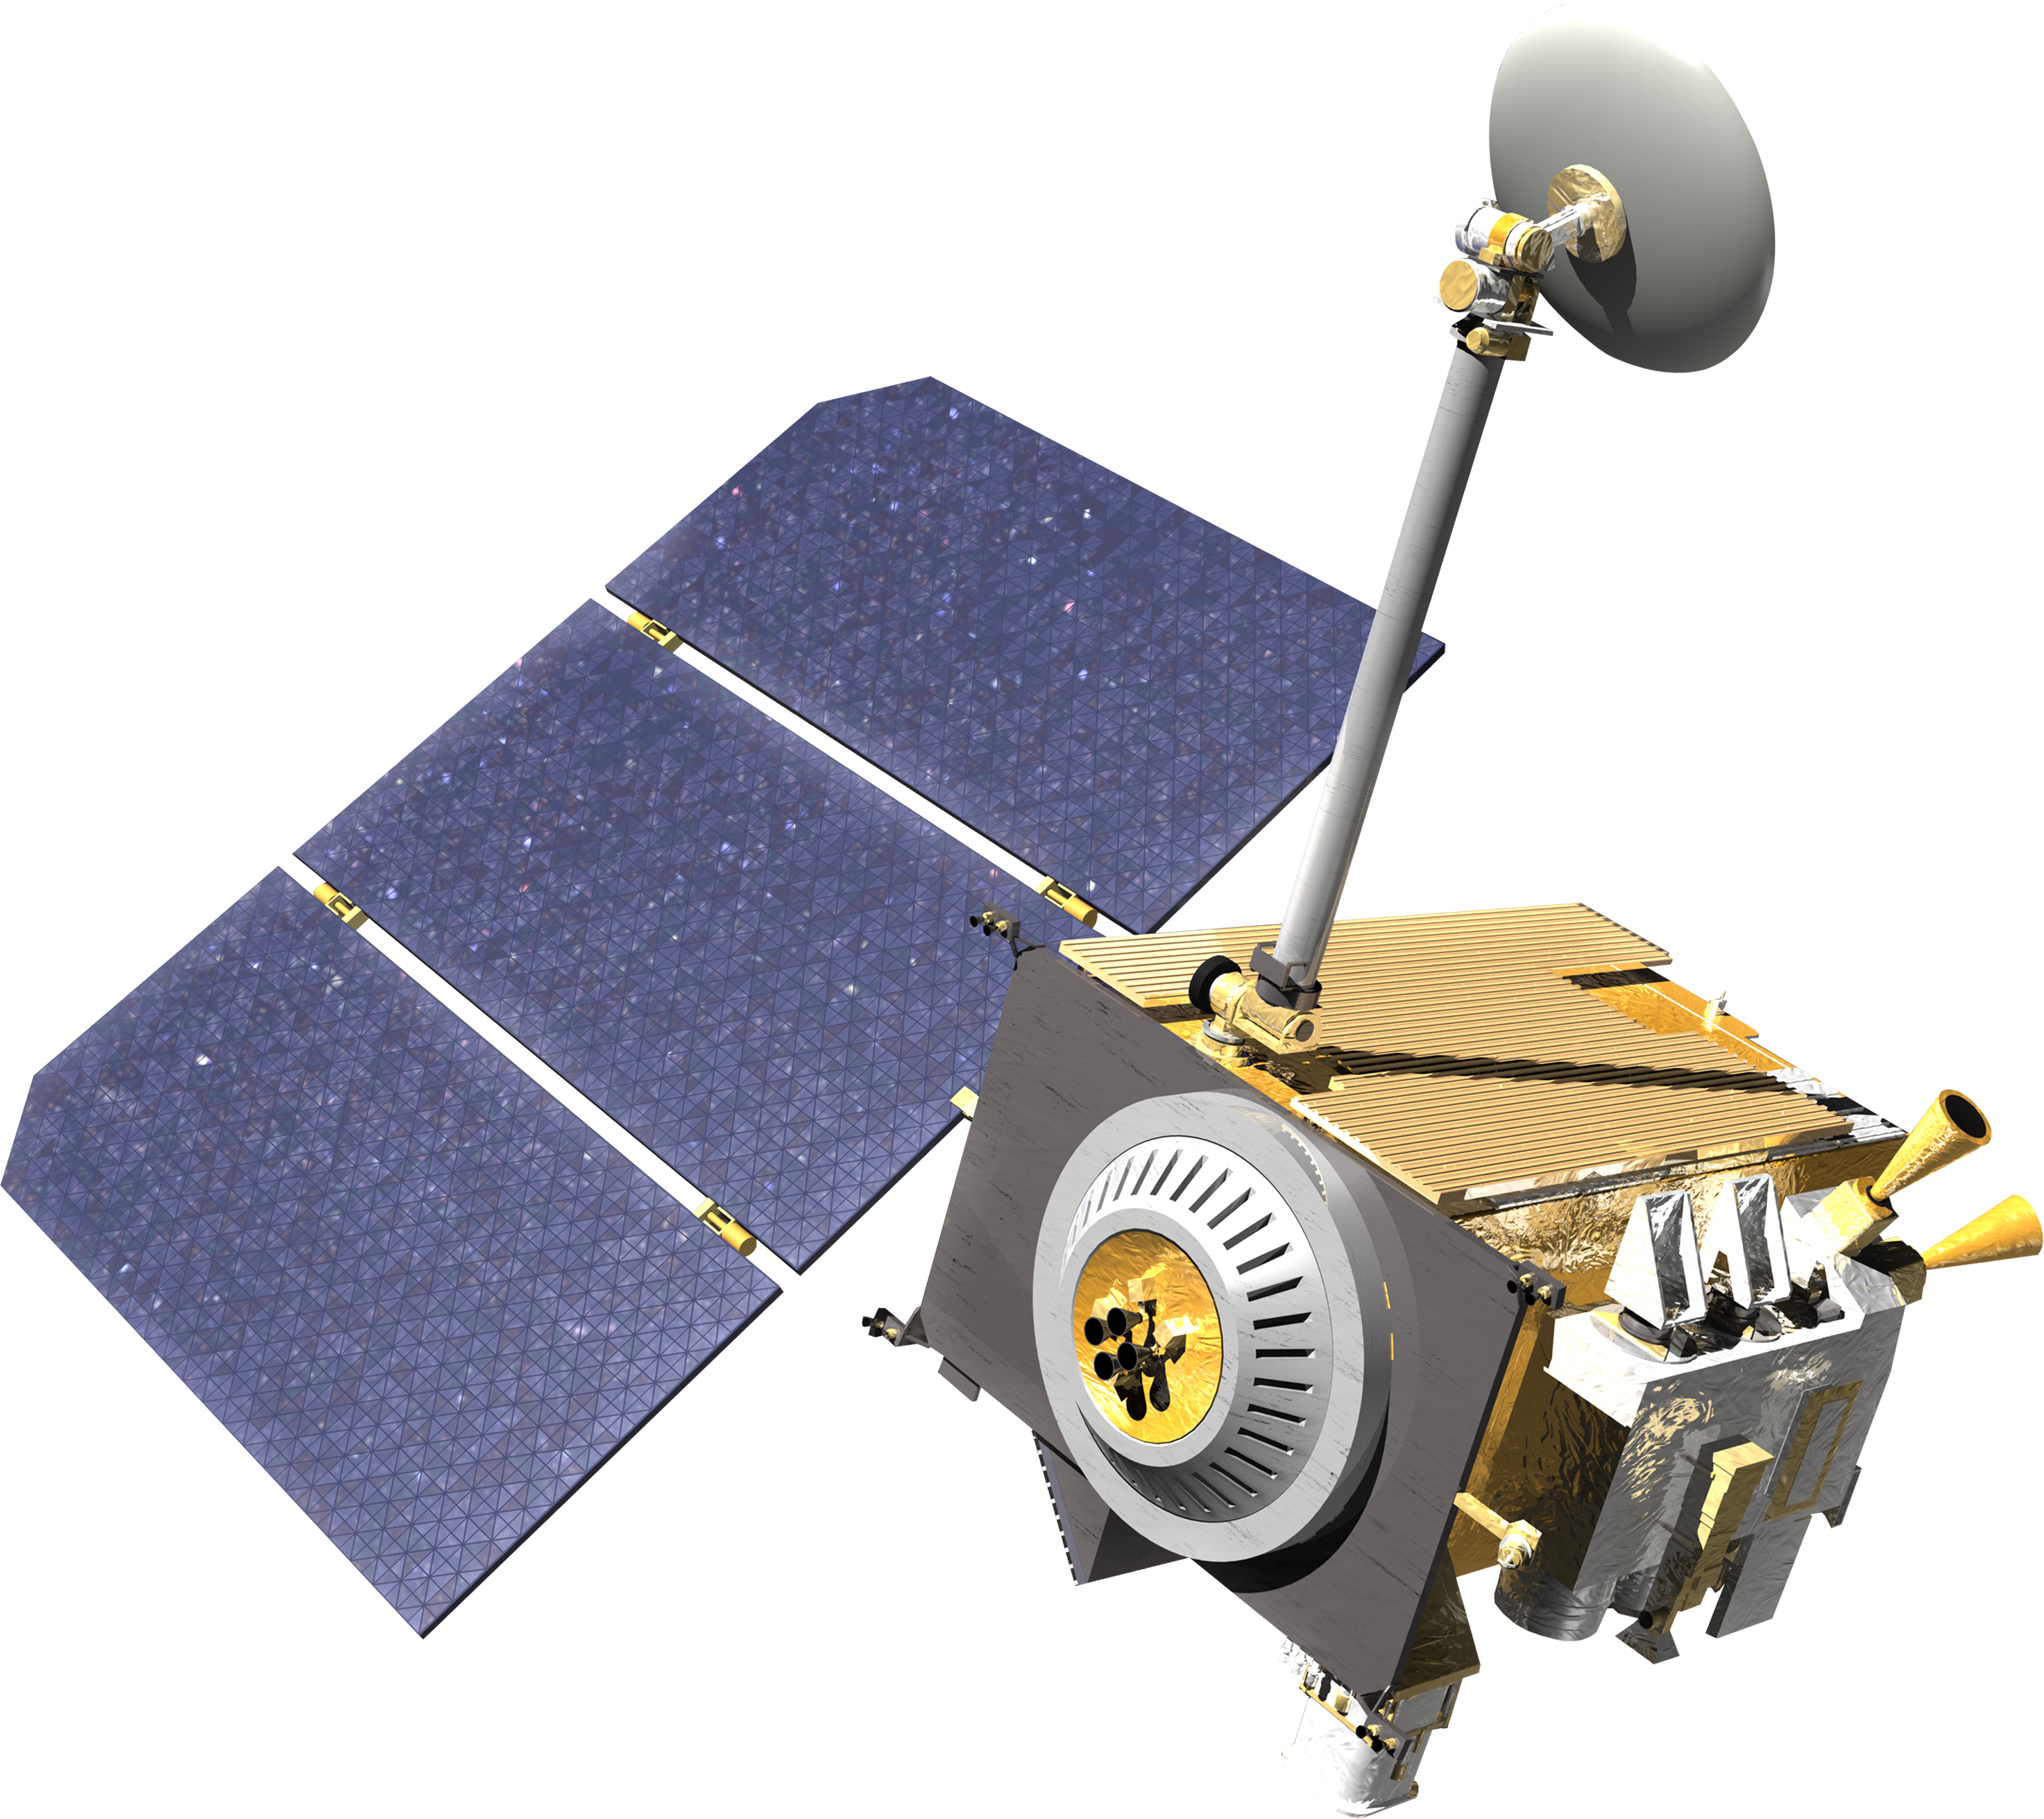
\includegraphics[width=\linewidth]{figures/lro_rendering.ai}
    \caption{Rendering of \gls{LRO}~\cite{NSMD2018} including bus frame definition. The X axis is along the velocity vector, the +Y axis is the anti-sun side, and the +Z axis is in the nadir direction~\cite{Tooley2010}.}
    \label{fig:lro-rendering}
\end{figure}

\gls{LRO} consists of a cubical bus with a large solar array and a protruding high gain antenna (\cref{fig:lro-rendering}). The solar array tracks the Sun in two axes, and the antenna points towards Earth whenever it is visible. This leads to large variations in cross-section over time, and different sides are presented to incoming solar and lunar radiation.


\begin{table}[b]
    \centering
    \caption{Panels for \gls{LRO} target model from \citeauthor{Smith2008}~\cite{Smith2008}. The coefficients are for absorptivity and specular/diffuse reflectivity. The solar array is by far the largest surface, followed by the Z-facing panels.}
    \label{tab:target-model}
    \begin{tabular}{lrrrr}
\toprule
\bfseries Panel & \bfseries $\mathbf C_a$ & \bfseries $\mathbf C_s$ & \bfseries $\mathbf C_d$ & $\mathbf A$~[\unit{\meter\squared}] \\
\midrule
\bfseries +X & 0.49 & 0.29 & 0.22 & 2.82 \\
\bfseries -X & 0.42 & 0.39 & 0.19 & 2.82 \\
\bfseries +Y & 0.45 & 0.32 & 0.23 & 3.69 \\
\bfseries -Y & 0.50 & 0.32 & 0.18 & 3.69 \\
\bfseries +Z & 0.50 & 0.32 & 0.18 & 5.14 \\
\bfseries -Z & 0.28 & 0.54 & 0.18 & 5.14 \\
\bfseries +SA & 0.90 & 0.05 & 0.05 & 11.00 \\
\bfseries -SA & 0.50 & 0.30 & 0.20 & 11.00 \\
\bfseries +HGA & 0.54 & 0.18 & 0.28 & 1.00 \\
\bfseries -HGA & 0.93 & 0.02 & 0.05 & 1.00 \\
\bottomrule
\end{tabular}

\end{table}

\gls{LRO} can be modeled as paneled target (\cref{eq:paneled-target}) to account for this variability. The panels are summarized in \cref{tab:target-model}. There are six panels for the bus, with surface normals along the positive and negative axes of the \gls{LRO} bus frame (cf. \cref{fig:lro-rendering}). The solar array and high gain antenna are modeled separately, again with frontside and backside panels. The solar array is almost as large as all other panels combined. Since it always points towards Sun, the solar \gls{RP} will have a large effect. Note that, while tracking of the solar array and antenna are constrained to two axes in reality, we allow three-axis tracking for simplicity. The definitive attitudes of both are also available but were not used since their data volume is prohibitively large. We also neglect self-shadowing, which was shown to only have a minor impact in most cases~\cite{Slojkowski2015,Loecher2018}, but can be significant for solar radiation~\cite{Mazarico2009}.

We also model \gls{LRO} as a cannonball (\cref{eq:cannonball-target}), a model which is often used for orbit determination. Finding a single equivalent cross-section area $A_c$ and \gls{RP} coefficient $C_r$ is virtually impossible~\cite{Vallado2013}. Different values for \gls{LRO} exist in literature: \citeauthor{Bauer2016} use $A_c = \qty{10}{\m\squared}$ and $C_r = 1.2$~\cite{Bauer2016}, while \citeauthor{Nicholson2010} use $A_c=\qty{14}{\m\squared}$ and $C_r = 1.0$~\cite{Nicholson2010}. Their acceleration should differ by about \qty{15}{\percent}. We choose the latter since it is used for operational orbit estimation of \gls{LRO}.

\begin{figure}[t]
    \centering
    \includegraphics[width=\linewidth]{figures/plots/mass_history.pdf}
    \caption{Mass evolution of \gls{LRO} over the science mission phase (15 September 2009 -- 11 December 2011, \textcolor[RGB]{206, 211, 217}{\ding{110}}). }
    \label{fig:mass-history}
\end{figure}

To complete the target model, the mass is required to convert forces into accelerations. \gls{LRO} performed monthly station keeping maneuvers during its science mission phase, which reduced the initial mass after science orbit insertion from \qty{1272}{kg} to \qty{1087}{kg} (\cref{fig:mass-history}). With every maneuver, \qty{6.3}{kg} of propellant are expelled~\cite{Mesarch2010}. This increases accelerations by \qty{15}{\percent} over the course of 21 months. To facilitate comparison and obtain worst-case results, we will use the end-of-mission mass of \qty{1087}{kg} in this paper, independently of the actual arc.





\subsection{LRO orbit geometry}

\begin{table}[b]
    \centering
    \caption{Orbit geometry for selected arcs over 2.5 days. The June arc gives full illumination, the September arc the maximum eclipse duration.}
    \label{tab:orbit-geometry}
    \begin{tabularx}{\linewidth}{Xrrr}
        \toprule
        & \bfseries 28 June 2010 & \bfseries 26 Sept. 2011 \\
        \midrule
        \bfseries $\mathbf \beta$~[\unit{\degree}] & \numrange{88.8}{88.9} & \numrange{-1.71}{-3.56} \\
        \bfseries Sun distance~[\unit{\astronomicalunit}] & 1.019 & 1.000 \\
        \bfseries Eclipse time~[\unit{\min}] & 0 & 48 \\
        \bottomrule
    \end{tabularx}
\end{table}

\gls{LRO}'s polar science mission orbit has a low altitude of \qty{50 \pm 15}{km}. The difference between periselene and aposelene is mostly due to a slight eccentricity, but also due to an equatorial radios that is \qty{2}{\km} larger than the polar radius. The altitude variation affects the lunar irradiance received by \gls{LRO}. The spacecraft has a period of \qty{113}{\min}.

Visibility of the Sun is determined by the beta angle $\beta$, which is the angle between the orbital plane and the Moon-to-Sun vector. It is zero when the Sun is within the plane and \qty{\pm 90}{\degree} when the orbit normal points towards the Sun. Since \gls{LRO}'s orbit is polar, it undergoes all $\beta$ within a year. For $\beta = \qty{0}{\degree}$, \gls{LRO} is moving towards and away from the Sun above the polar, experiences the maximum eclipse duration, and passes over the subsolar point.  For $\beta = \qty{90}{\degree}$, \gls{LRO} is in full view of the Sun throughout the orbit, and there is no along-track component of the solar radiation. The spacecraft does not pass over hot or well-illuminated lunar regions.

Since the effect of \gls{RP} varies greatly with $\beta$, we will investigate two arcs in this paper. They are summarized in \cref{tab:orbit-geometry}. In June, Moon is at aphelion and no eclipses occur. In September, the beta angle is just below \qty{0}{\degree}; \gls{LRO} will experience the maximum solar eclipse duration of \qty{48}{\min}. No lunar eclipses occur during any of the arcs. Both arcs have a length of 2.5 days, which is used for orbit determination of \gls{LRO}~\cite{Nicholson2010,Mazarico2011}. Choosing the same length ensures our results are relevant for error estimation in force modeling for orbit determination.




\subsection{Simulation setup}

simulation setup in table, explanations in text

earth albedo + thermal radiation can be neglected for LRO since it is less than 0.1\% of solar radiation at moon

solar array tracks Sun, HGA tracks Earth~\cite{Tooley2010}
start at start at 26 June 2010 06:00:00
Earth eclipses Sun during this time
Moon does not eclipse Sun (Sun beta angle is about -90 deg, see~\cite{Tooley2010})

occultations
lunar eclipses avoided since we cannot represent multiple occultations

effects of neglecting terrain and self shadowing~\cite{Mazarico2018} sec 4.2 and 4.3


Operational LRO OD does not use lunar albedo due to computational demand, but used for offline reprocessing.
Self-shadowing from \citeauthor{Mazarico2009} is used for reprocessing~\cite{Nicholson2010}

step 5 s, which is also used for LRO orbit determination~\cite{Mazarico2018}

MOON\_PA frame, IAU\_MOON is in worst case 155 m off~\cite{NAIF2020} (Special PCK and FK for Earth and Moon, slide 14)

integrator + propagator params



two arcs, one for beta = 0 and beta = 90
describe why These